%=======================+=========================
%================  Introduction  ================
%=================================================
\section[The \gx{} experiment (Curtis)]{\label{sec:gluexexperiment} The \gx{} experiment}
The search for QCD exotics has been on going for several decades and utilizes data from a wide range of experiments and production mechanisms. Historically, such searches have looked for gluonic excitations of mesons, looking for both states of pure glue, glueballs, and those where the gluonic field binding the quark-anti-quark pair has been excited, hybrid mesons. Reviews of searches for glueballs~\cite{Crede:2008vw} show that most of these looked for so-called scalar glueballs, where the searches rely on over population of nonets as well as unusual decay patterns of the states. In the search for hybrid mesons~\cite{Meyer:2010ku,Meyer:2015eta}, searches have focused on states with non-quark-anti-quark (exotic) quantum numbers and good evidence exists for an isospin $1$ state, the $\pi_{1}(1600)$. Looking collectively at past studies, we find that data from high-statistics photoproduction experiments in the relevant energy regime is lacking. 

\begin{figure}[h!]\centering
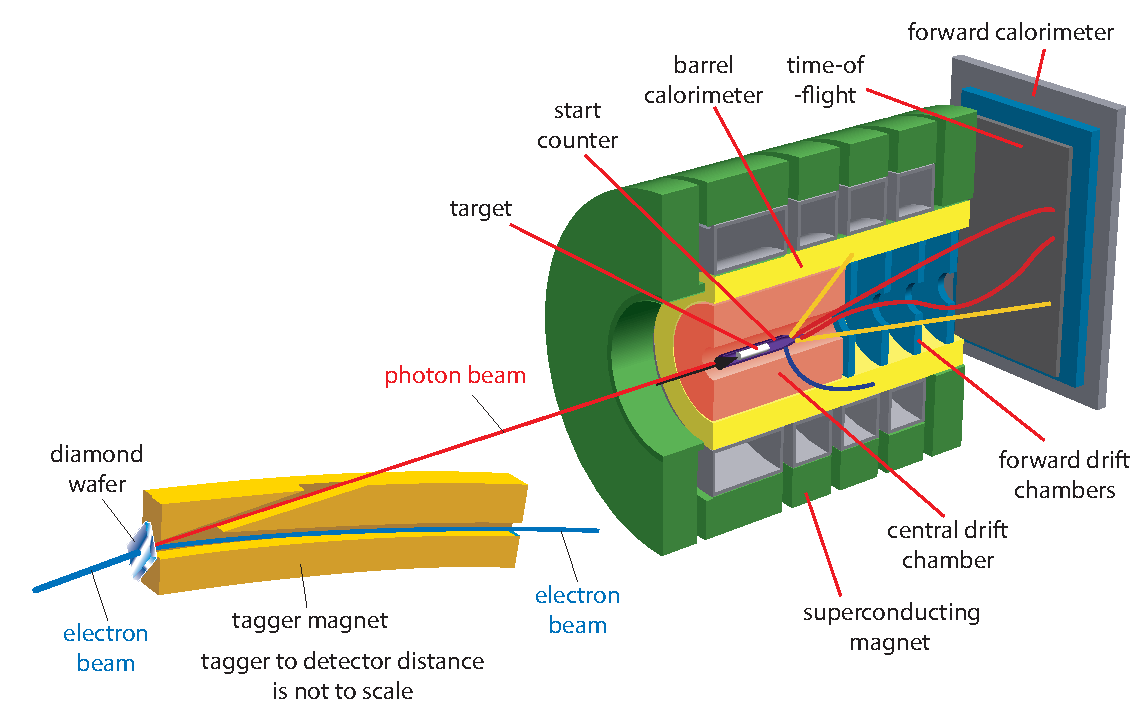
\includegraphics[width=0.75\textwidth]{figures/detector_beamline_noplug_noGlueX.pdf}
\caption[]{\label{fig:gluex_cut-away}(Color online)A cut-away drawing of the \GX{} detector in Hall D.}
\end{figure}
The \gx{} experiment at Jefferson Lab has been built to both search for, and map out the spectrum of exotic hybrid mesons using a high-energy (9~GeV) linearly-polarized photon beam incident on a proton target\cite{gluex-ref}. The detector is nearly hermetic for both charged particles and photons, allowing for reconstruction of exclusive final states. A 2~T solenoidal magnet surrounds the drift-chamber based tracking. Two electromagnetic calorimeters cover the central and forward regions, and a scintillation detector down stream provides particle-identification capability through time-of-flight measurements. The \gx{} detector and beamline is shown schematically in Figure~\ref{fig:gluex_cut-away}.


\subsection[The Hall D complex]{The Hall D complex \label{sec:gluexexperiment:complex}}
The \gx{} experiment is housed in the Hall D complex at Jefferson Lab. This new construction starts with an extracted electron beam at the north end of the Continuous Electron Beam Accelerator Facility (CEBAF). These are the highest-energy electrons at the lab, up to 12~GeV, due to the extra one-half pass of acceleration they have relative to the other experimental areas. The electron beam enters the tagger hall where it is used to produce linearly polarized photons through coherent bremsstrahlung~\cite{} on a 50~$\mu$m thick diamond crystal radiator. The scattered electrons pass through a tagger magnet and are bent into tagging detectors. A high-resolution array consisting of scintillating fibers covers the 8 to 9~GeV energy range, and a tagger hodoscope covers photon energies both from 9~GeV to the endpoint, and down from 8~GeV to 3~GeV. Those electrons not interacting in the diamond are directed into a 60 kW electron-beam dump. The tagged photons pass through a tunnel to the Hall-D experimental hall. The distance from the radiator to the 5~mm diameter primary collimator, which removes the off-axis incoherent photons, is 75 m. The from face of the collimator is instrumented with an active collimator to aid in beam tuning. 

Downstream of the collimator is a thin beryllium radiator used by both the triplet polarimeter which measures the linear polarization of the photons and a pair spectrometer which is used to measure the flux of the photons. More information on the production, tagging and monitoring of the photon beam can be found in Section~\ref{sec:beamline}. The photons then pass through a 30~cm long liquid hydrogen target at the heart of the \gx{} detector. Photons which did not interact in the target travel to the end of the experimental hall where they enter the photon beam dump.

The \gx{} detector is based on a 4~m long solenoidal magnet which is operated at a maximum field of 2~T. A sketch of the detector is shown in Fig.~\ref{fig:gluexsketch}, while more information on the solenoid is in Section~\ref{sec:solenoid}. The liquid-hydrogen target is located 65~cm inside the upstream bore of the magnet. It consists of a 2~cm diameter, 30~cm long volume of hydrogen and is described in Section~\ref{sec:target}. Surrounding the target is the start counter which consists of 30 thin scintillator paddles that bend to a nose on the down-stream end of the target. The start counter is primary detector that identifies the radio-frequency (RF) bunch that contained the incident electron. More information can be found in Section~\ref{sec:scintillators}. 
\begin{figure}[htbp]\centering
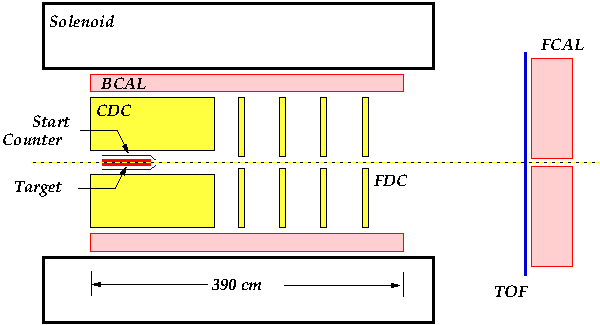
\includegraphics[width=0.7\textwidth]{figures/GlueX_Sketch.pdf}  
\caption{\label{fig:gluexsketch} (Color online)         
Sketch of GlueX detector.  The main systems of the detector are the Start Counter \cite{Pooser:2019rhu}, the Central Drift Chamber (CDC) \cite{VanHaarlem:2010yq} the Forward Drift Chamber (FDC) \cite{Pentchev2017281}, a scintillator-based Time of Flight (TOF) wall and a lead-glass Forward Calorimeter (FCAL) \cite{MORIYA201360}. The Barrel Calorimeter (BCAL) is sandwiched between the drift chambers and the inner radius of the solenoid.}   
\end{figure}

Starting at a radius of 10~cm from the beam line is the central drift chamber, a cylindrical straw-tube detector. The active volume of the chamber extends from 48~cm upstream to 102~cm downstream of the target center, and from 10~cm to 56~cm in radius. It consists of 28 layers of straw tubes in both axial and two stereo orientations. Downstream of the central tracker is the forward drift chamber. This device consists of four packages, each containing 6 planar layers in alternating $u$-$y$-$v$ orientations. Both cathodes and anodes are readout from the forward chambers, providing 3D space point measurements. More details on the tracking system can be found in Section~\ref{sec:tracking}. 

Downstream of the magnet is the time-of-flight wall. The detector consists of two layers of scintillator paddles in a crossed pattern, and in conjunction with the start counter, is used to measure the flight-time of charged particles. More information can be found in Section~\ref{sec:scintillators}. 
Photons in \gx{} are detected in two calorimeter systems. The barrel calorimeter, located inside the solenoid, consists of layers of scintillating fibers alternating with lead sheets. The forward calorimeter is downstream of the time-of-flight wall, and consists of $2800$ lead-glass blocks. More information can be found in Section~\ref{sec:calorimeters}.

\subsection[Experimental Requirements]{Experimental Requirements \label{sec:intro:requirements}}
In order to exclusively reconstruct final states, the \gx{} detector needs to be able to reconstruct both charged particles, $\pi^{\pm}$, $K^{\pm}$ and $p$, and particles decaying into photons, $\pi^{\circ}$, $\eta$, $\omega$ and $\eta^{\prime}$. For this, the charged particles and photons must reconstructed with good momentum and energy resolution. The experiment also needs to be able to reconstruct the incident photon's energy (8 to 9~GeV) with high accuracy ($0.1$\%) and know its degree of linear polarization (40\%) at the percent-level. Finally, many of the interesting final states involve more than five particles in their final state. Thus, the \gx{} detector must also be nearly hermetic for both charged particles and photons, with an acceptance that is reasonably uniform, well understood and accurately modeled in simulation.

Typical momentum resolution for charged particles $1$--$3\%$, while for very-forward high-momentum particles, it is somewhat worse at around $8$-$9\%$. For most charged particles, the tracking system has nearly hermetic acceptance for polar angles in the lab from about $1-2^{\circ}$ to $150^{\circ}$. Because of the target thickness, protons with momentum below about 250~MeV/c are not detected, and pions with momentum under 200~MeV/c can have spiraling trajectories in the detector, making reconstruction challenging. $dE/dx$ in the central drift chamber can separate pions and protons up to about 800~MeV/c, while time-of-flight can separate forward-going pions and kaons up to about 2~GeV/c.

For photons, the typical energy resolution is 5 to 6\%$/\sqrt{E_{\gamma}}$. There is some variation in the barrel calorimeter resolution, depending on the incident angle of the photon, but generally, photons above about 60~MeV can be detected in the barrel calorimeter. The interaction point along the beam direction is determined by comparing the information from the readouts on the upstream and downstream ends of the detector. The forward calorimeter can reconstruct photons whose energy is larger than 100~MeV, with uniform resolution across the face of the detector. There is a gap region between the calorimeters at around $11^{\circ}$, where energy can be lost due to leakage. Both photon-detection efficiency and energy resolution are degraded in this region. 
 
\subsection{Data Requirements \label{sec:intro:data_requirements}}
To be able to carry out the necessary analyses in small bins of energy and momentum transfer, $t$, the detector not only must have the ability to reconstruct exclusive final states but also collect sufficient statistics. Thus, the \GX{} experiment is also a high-statistics experiment. While exact cross sections are not known, it is expected that those of interest will be in the 10~nb range, with the largest cross sections of interest are 1~$\mu$b. The initial phase of the \GX{} experiment has run with a data acquisition system capable of collecting data using photon beams with a few $10^{7}~\gamma/$s in the coherent peak (8.4-9 GeV), while the expectation is to run about 2.5 times higher rates going forward. The data acquisition ran routinely at 40\,kHz with raw event sizes of $15-20$kilobytes, collecting about 600~megabytes of data per second. With trigger improvements, future running is expected at about 90 kHz and about 1~gigabyte per second.  

\subsection{Coordinate system \label{sec:intro:coordinates}}
We introduce the overall experiment coordinate system, which is used in this document and throughout the analysis. The experimental area is located 
off the north east corner of the accelerator. The z-axis is defined along the nominal beamline increasing downstream (toward the east). The coordinate system 
is right-handed with the y-axis pointing vertically up and the x-axis pointing approximately north. 
The origin is located 50.8\,cm (20 inches) downstream of the upstream side of the upstream endplate of the solenoid. That places the nominal center of the target at (0,0,65\,cm).
